\section{Snímky obrazovky z aplikace}
\textit{Tato sekce obsahuje snímky z aplikace a velmi stručný návod na její obsluhu. Cílem této sekce není poskytnutí uživatelské dokumentace. Pouze popisuje její základní principy.}

Po spuštění aplikace je uživatel vyzván k výběru konfigurace. V tomto okně je také možné zadat IRI konfigurace a meta konfigurace ručně, nebo otevřít existující graf ze souboru. Jakmile je uživatelem vybrána konfigurace, je vyzván k výběru prvního vrcholu, který bude přidán do grafu. To je možné provést ze seznamu předdefinovaných vrcholů, nebo může použít vyhledávací pole.

Hlavní okno aplikace má uprostřed grafovou oblast. S tou je možné manipulovat pomocí myši, nebo červených tlačítek v pravém dolním rohu. Po kliknutí na vrchol, označení více vrcholů, nebo skupiny se zobrazí pravý boční panel s detailními informacemi. Levý panel se automaticky skrývá a obsahuje další akce, které je možné s grafem provést. V levém horním rohu se také nachází pole, přes které lze přidávat a vyhledávat vrcholy v grafu.

\begin{figure}[h]
    \centering
    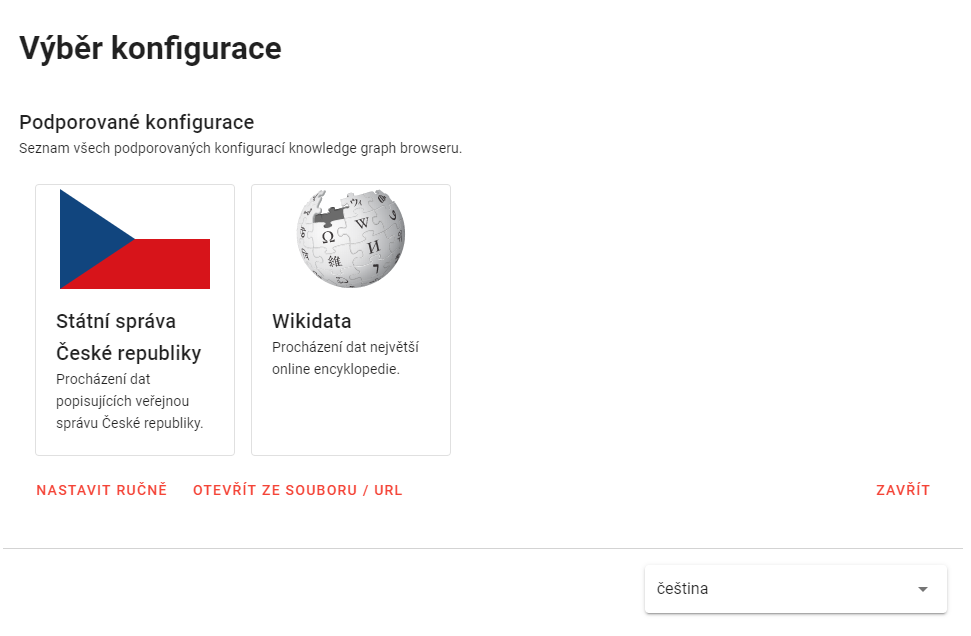
\includegraphics[width=\textwidth]{media/metaconfiguration.png}\\
    \caption{Úvodní obrazovka s výběrem mezi dvěma meta konfiguracemi. Je také možné ručně zadat IRI konfigurací nebo stáhnout graf ze souboru.}
\end{figure}

\newpage

\begin{figure}
    \centering
    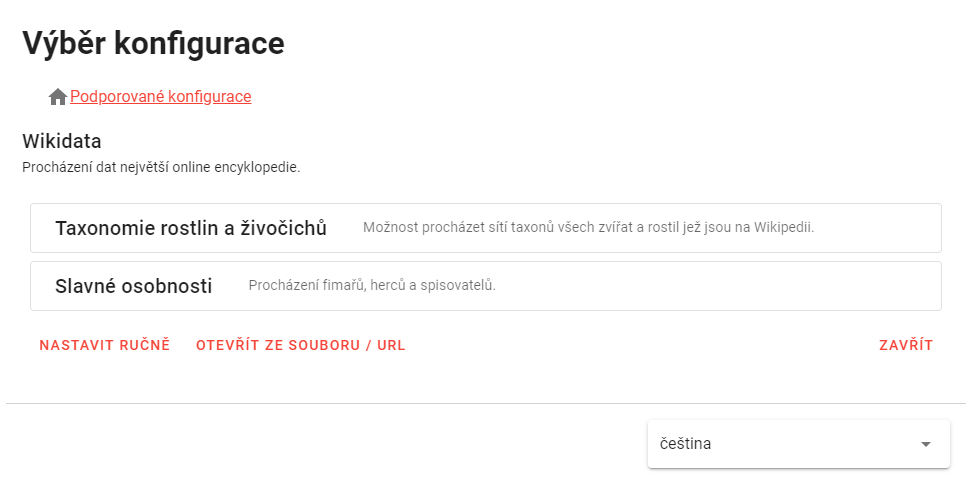
\includegraphics[width=\textwidth]{media/configuration.png}
    \caption{Obrazovka s výběrem konkrétních konfigurací v rámci Wikipedie (Wikidat).}
    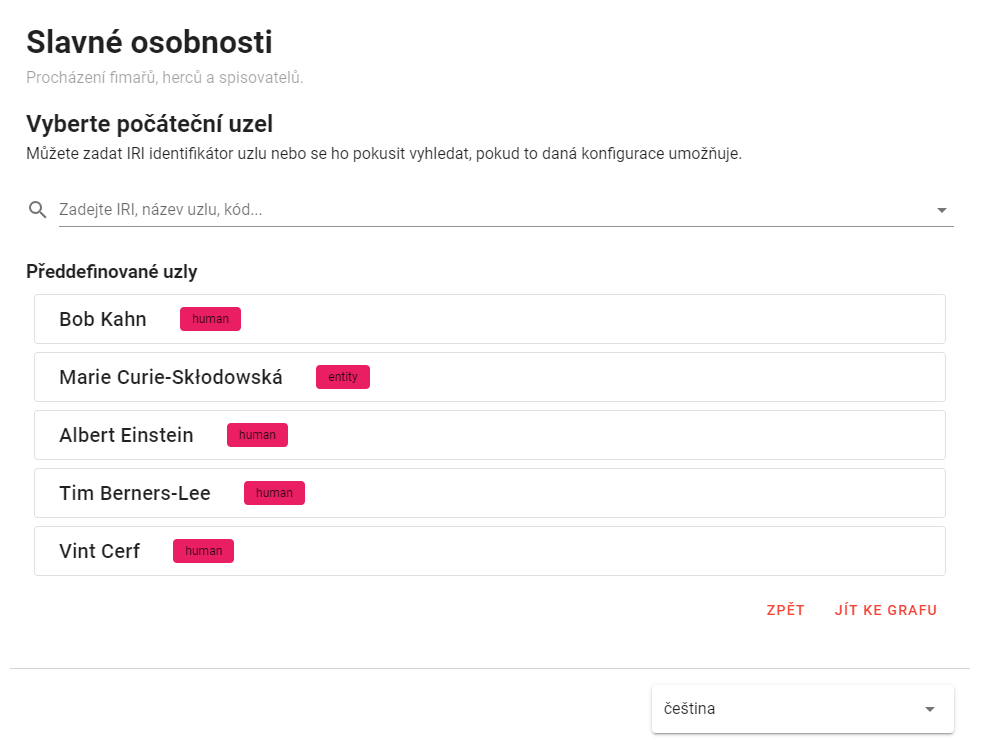
\includegraphics[width=\textwidth]{media/node-selection.png}
    \caption{Obrazovka s výběrem počátečního vrcholu. Ten je možné vybrat z předdefinovaných, nebo je možné použít vyhledávací pole.}
\end{figure}

\newpage

\begin{figure}
    \centering
    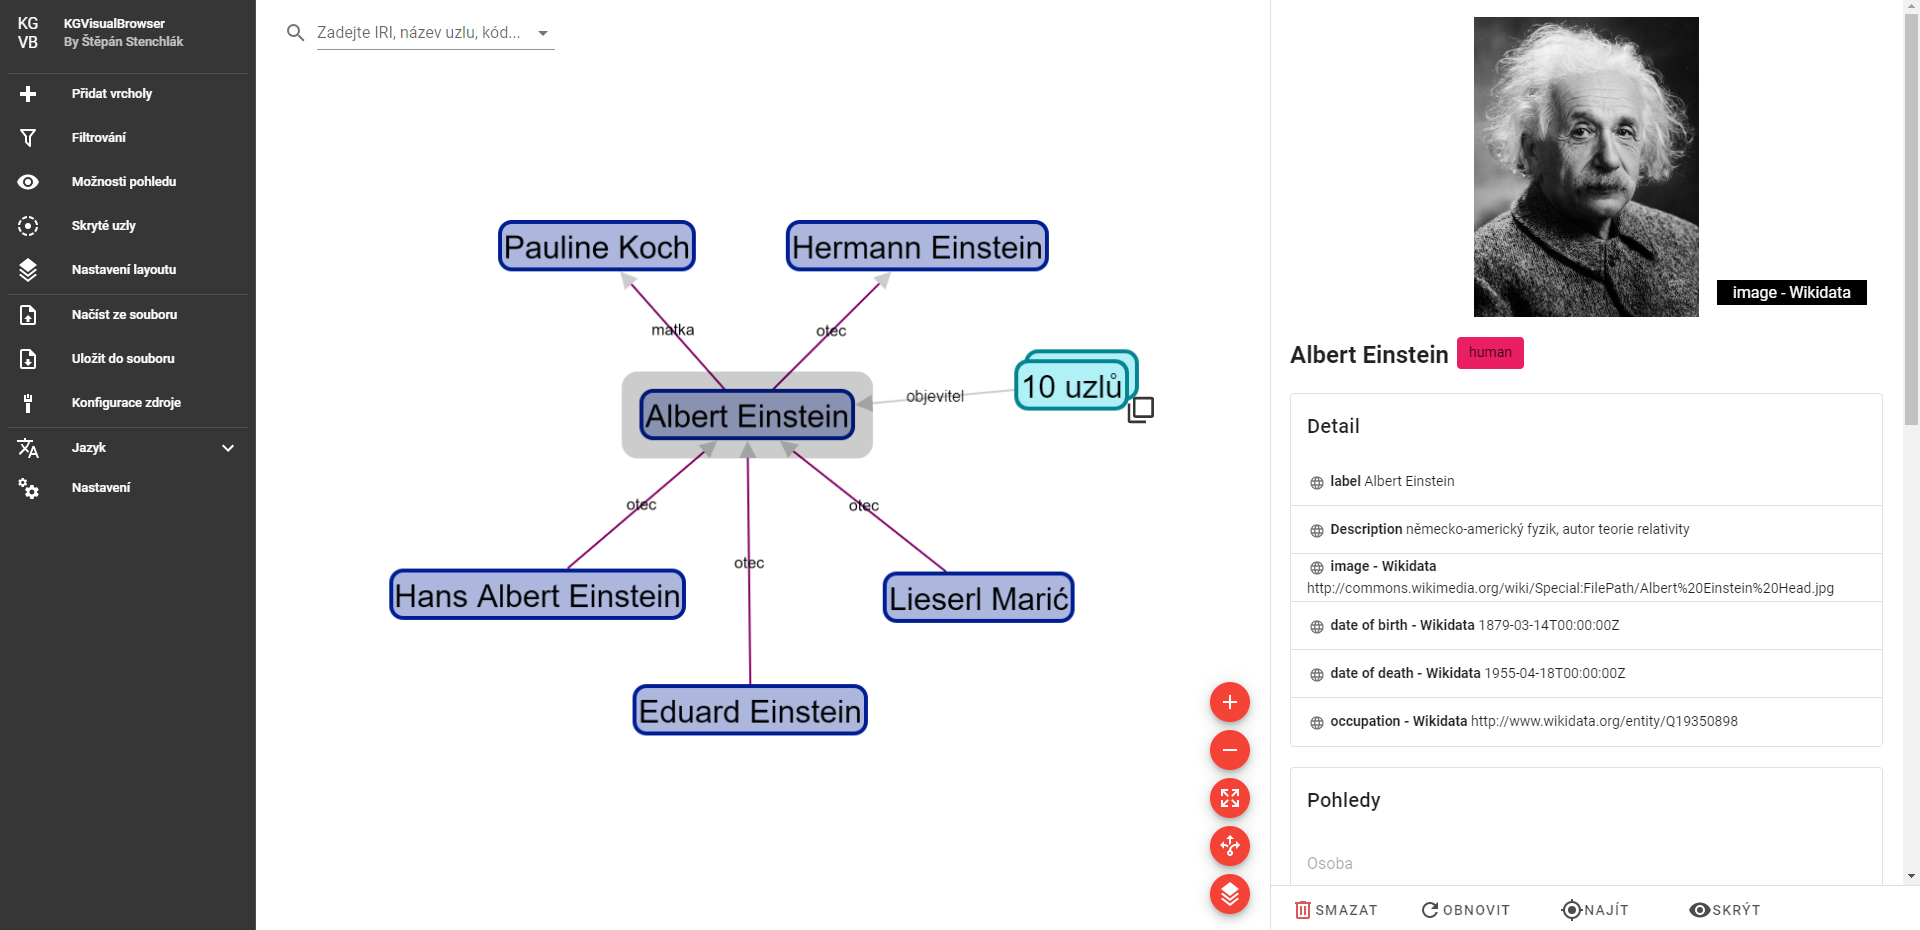
\includegraphics[width=\textwidth]{media/einstein.png}
    \caption{Hlavní okno aplikace s již načteným grafem a vybraným vrcholem. Levý panel je zde rozevřený.}
    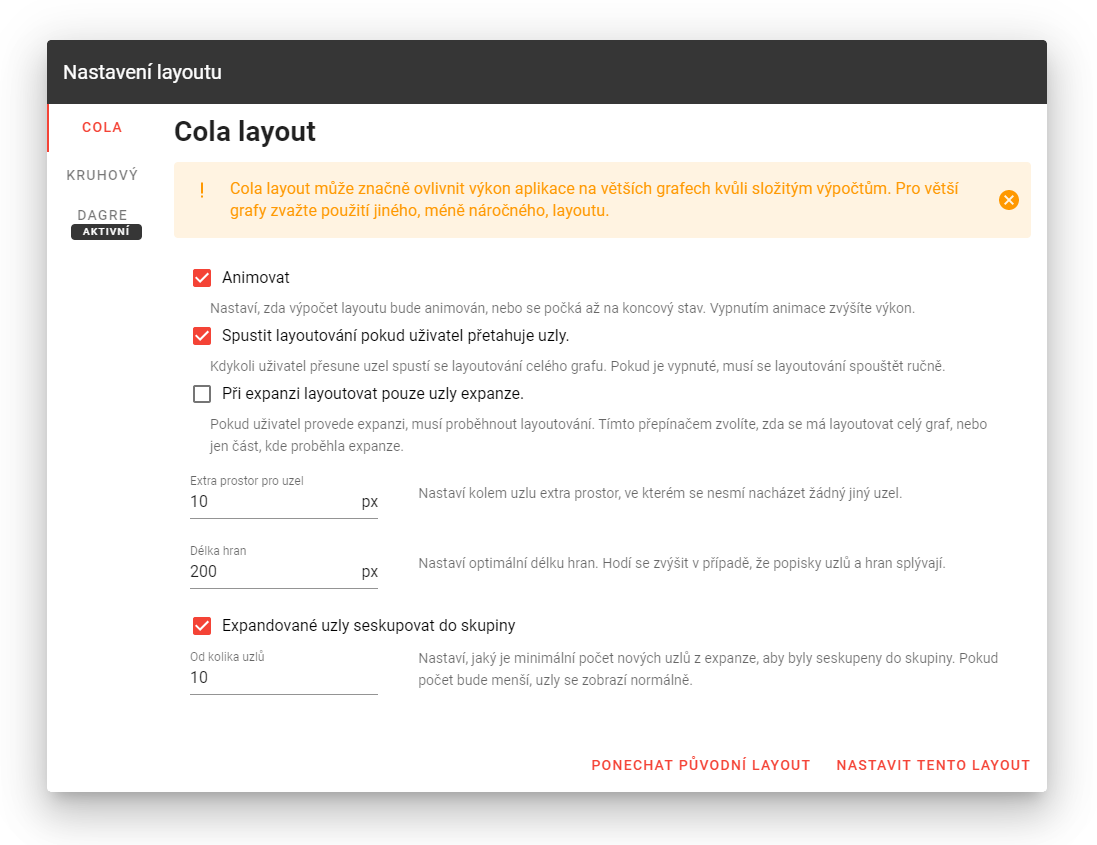
\includegraphics[width=\textwidth]{media/layout.png}
    \caption{Dialog pro výběr a nastavení layoutů.}
\end{figure}